\begin{figure}
    \centering
    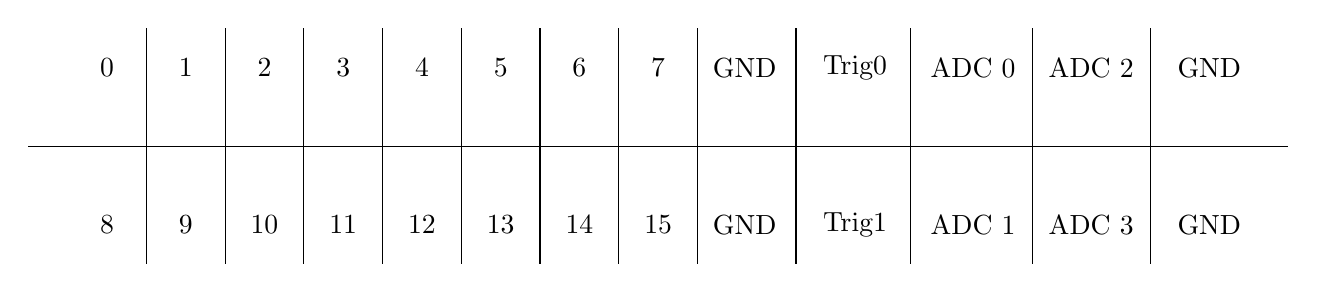
\begin{tikzpicture}
        \draw
            (-1, 0) -- (15, 0)

            (0, 1) node[]{0}
            (1, 1) node[]{1}
            (2, 1) node[]{2}
            (3, 1) node[]{3}
            (4, 1) node[]{4}
            (5, 1) node[]{5}
            (6, 1) node[]{6}
            (7, 1) node[]{7}

            (0, -1) node[]{8}
            (1, -1) node[]{9}
            (2, -1) node[]{10}
            (3, -1) node[]{11}
            (4, -1) node[]{12}
            (5, -1) node[]{13}
            (6, -1) node[]{14}
            (7, -1) node[]{15}

            (8.1, 1) node[]{GND}
            (8.1, -1) node[]{GND}

            (9.5, 1) node[]{Trig0}
            (9.5, -1) node[]{Trig1}

            (11, 1) node[]{ADC 0}
            (11, -1) node[]{ADC 1}
            (12.5, 1) node[]{ADC 2}
            (12.5, -1) node[]{ADC 3}
            (14, 1) node[]{GND}
            (14, -1) node[]{GND}
        
            (0.5, 1.5) -- ++ (0, -3)
            (1.5, 1.5) -- ++ (0, -3)
            (2.5, 1.5) -- ++ (0, -3)
            (3.5, 1.5) -- ++ (0, -3)
            (4.5, 1.5) -- ++ (0, -3)
            (5.5, 1.5) -- ++ (0, -3)
            (6.5, 1.5) -- ++ (0, -3)
            (7.5, 1.5) -- ++ (0, -3)
            (8.75, 1.5) -- ++ (0, -3)
            (8.75, 1.5) -- ++ (0, -3)
            (10.2, 1.5) -- ++ (0, -3)
            (11.75, 1.5) -- ++ (0, -3)
            (13.25, 1.5) -- ++ (0, -3)
        ;
    \end{tikzpicture}
    \caption{Pin header}
    \label{figure:pin_header}
\end{figure}